\documentclass[11pt]{article}

\usepackage[utf8]{inputenc}
\usepackage[T1]{fontenc}
\usepackage[margin=2.5cm]{geometry}
\usepackage{graphicx}
\usepackage{siunitx}
\usepackage{hyperref}
\usepackage{tcolorbox}
\usepackage{booktabs}
\usepackage{amsmath}

\tcbuselibrary{skins}

\newtcolorbox{pending}{
  colback=yellow!10, colframe=yellow!60!black,
  boxrule=0.6pt, arc=2pt, left=6pt, right=6pt, top=4pt, bottom=4pt,
  title={Pending}, fonttitle=\bfseries\small, coltitle=black
}

\title{Hot-Swap eFuse (LTC4215) --- Digital Telemetry Front-End \\ \large STM32F411CEU6 over I\textsuperscript{2}C}
\author{IKGB105}
\date{\today}

\begin{document}
\maketitle

% ======================================================================
\section{Project Objective}

\texttt{EFUSE\_LTC4215} (the project this one extends) deliberately left the LTC4215's
I\textsuperscript{2}C/SMBus monitoring interface unused -- every ADR/SCL/SDA pin was wired
no-connect, and the datasheet's onboard ADC (current, voltage, fault status) was flagged in that
project's own \emph{Known Limitations} as "real LTC4215 features left entirely untested here."

This project closes that gap: it adds a minimal STM32F411CEU6 system to the same board, wired to
the LTC4215's I\textsuperscript{2}C bus, turning the eFuse from a purely analog hot-swap/protection
circuit into one with digital telemetry read-out. It is the Phase 3 "digital power monitoring" item
of the broader hardware roadmap (hot-swap $\to$ digital power/PMBus-style monitoring $\to$ PDN
analysis), chosen specifically because the LTC4215's monitoring interface was already sitting there
unused rather than as a new, unrelated MCU exercise.

Scope, same convention as every project in this series: \textbf{simulation + schematic + PCB layout
only, not physically built}. A COMSOL thermal FEM was already carried out for the eFuse power stage
in \texttt{EFUSE\_LTC4215}; this project does not repeat it (Section~\ref{sec:scope-thermal}).

\begin{pending}
Firmware (I\textsuperscript{2}C register read-out, compiled against the HAL but not flashed/tested
on real hardware) and a PDN (power distribution network) impedance-vs-frequency check of the 3.3\,V
rail are both still open -- see Section~\ref{sec:pending}.
\end{pending}

% ======================================================================
\section{MCU Selection}

\textbf{STM32F411CEU6} (UFQFPN48), the same part used on the WeAct "Blackpill" board. Chosen over a
smaller part (e.g.\ STM32F030) for two concrete reasons, not just familiarity:
\begin{itemize}
\item Direct USB 2.0 FS peripheral (OTG\_FS) for USB-DFU flashing, matching a workflow already known
  from the real Blackpill, without needing an external SWD programmer.
\item More compute/memory headroom than strictly required for I\textsuperscript{2}C register
  read-out, left available for a possible future command-parsing layer (closer to true PMBus-style
  interaction) without a second board respin.
\end{itemize}

The real WeAct Blackpill schematic (\texttt{docs/reference/}) was used as the primary layout
reference, cross-checked and corrected in several places -- documented as pitfalls in
Section~\ref{sec:pitfalls} rather than copied blindly.

% ======================================================================
\section{Design}

\subsection{I\textsuperscript{2}C integration with the LTC4215}
\label{sec:i2c}

The LTC4215's I\textsuperscript{2}C-related pins, all left unconnected in the original eFuse design,
are now wired per the datasheet (Rev E, "I\textsuperscript{2}C Interface" and pin function sections):

\begin{itemize}
\item \textbf{SDAI (pin 8) and SDAO (pin 7) tied together}, forming the single bidirectional SDA line
  -- the QFN package exposes them separately specifically to allow an optoisolator on SDAO alone; not
  used here, so they are simply shorted.
\item \textbf{SCL (pin 9)} to the bus directly.
\item \textbf{ADR0 (pin 12) and ADR2 (pin 14) tied to INTVCC}, \textbf{ADR1 (pin 13) left floating
  (No Connect)} -- reproducing the datasheet's own worked example (Figure 5): this combination sets
  I\textsuperscript{2}C address \textbf{19} (binary \texttt{1010011}), chosen for traceability to the
  datasheet rather than an arbitrary new value, since this is the only device on the bus and the exact
  address has no functional consequence.
\item \textbf{GPIO (pin 18)} kept as in the original design (power-good flag); \textbf{-ALERT (pin
  10)}, previously unused, now routed to the STM32 as an EXTI interrupt source.
\item Pull-ups: \textbf{\SI{4.7}{\kilo\ohm} on SCL and SDA}, \textbf{\SI{10}{\kilo\ohm} on ALERT} (slower interrupt
  line, no need to match the bus speed resistors), all to \textbf{INTVCC} ($\approx$\SI{3.1}{\volt}
  typ regulated, close enough to the STM32's 3.3\,V logic levels that no level shifter is needed --
  confirmed from the datasheet's own electrical table, not assumed).
\end{itemize}

\subsection{STM32 minimal system}

\begin{itemize}
\item \textbf{Power}: three VDD pins (24/36/48) and VSS at pins 23/35/47/49 (the last one being the
  UFQFPN48's exposed pad -- the default KiCad symbol represents it as a fourth, hidden VSS pin stacked
  on top of pin 23, electrically merged by position, not a separate net to manage; verified directly
  against the symbol library file, Section~\ref{sec:pitfalls}). VBAT tied directly to 3.3\,V with its
  own \SI{100}{\nano\farad} -- no RTC battery backup is implemented, so the WeAct reference's
  BAT54C diode-OR network was simplified away.
\item \textbf{VDDA/VREF+} filtered from 3.3\,V through a \SI{10}{\micro\henry} ferrite (L1) plus a
  bank of \SI{100}{\nano\farad} decoupling, isolating the ADC/PLL analog supply from digital switching
  noise.
\item \textbf{VCAP1 (pin 22)}: \SI{2.2}{\micro\farad}, required for the F4's internal 1.2\,V core
  regulator.
\item \textbf{Clock}: \SI{25}{\mega\hertz} crystal (Y2, \SI{9}{\pico\farad} load, 3225 SMD package)
  with \SI{12}{\pico\farad} loading caps on PH0/PH1 -- no 32.768\,kHz RTC crystal, intentionally
  dropped (Section~\ref{sec:pitfalls}).
\item \textbf{Reset / Boot}: NRST with \SI{100}{\nano\farad} only (the STM32 has an internal pull-up);
  BOOT0 with a \SI{10}{\kilo\ohm} pull-down plus a push-button to 3.3\,V to force USB-DFU entry;
  \textbf{BOOT1 (shared with PB2 on the F401/F410/F411/F412 value line, confirmed against RM0383)}
  likewise pulled down -- both are genuinely required on this part, not a copy-paste artifact from the
  F1 series (Section~\ref{sec:pitfalls}).
\item \textbf{USB-C}: D+/D- through \SI{10}{\ohm} series resistors to PA12/PA11; CC1 and CC2 each with
  their own independent \SI{5.1}{\kilo\ohm} pull-down to GND (two resistors, not one shared -- does
  not rely on the footprint shorting CC1/CC2 together); VBUS left unconnected -- the board is
  self-powered from +12V, not from the USB bus (PA9 is available for an optional VBUS-sense GPIO, not
  populated).
\item \textbf{SWD}: 4-pin header (3V3, SWDIO, SWCLK, GND).
\end{itemize}

\subsection{12\,V $\to$ 3.3\,V regulation}

A single linear stage, \textbf{LD1117S33TR (SOT-223)}, direct from the board's +12\,V rail -- not a
two-stage USB-VBUS-then-3.3V path like the real Blackpill, since this board's primary (and only)
power source is the eFuse's +12\,V input. A Schottky (D4, SS14) in series protects against reverse
input polarity.

Linear dissipation: $P \approx (12 - 0.4_{D4} - 3.3)\,\si{\volt} \times I$. At an estimated
\SI{50}{\milli\ampere} load (MCU + USB PHY idle, no heavy peripheral activity), $P \approx
\SI{0.42}{\watt}$ -- acceptable in a SOT-223 with modest copper pour as heatsink. If the 3.3\,V load
later grows past roughly \SI{120}{\milli\ampere}, a linear regulator stops being a reasonable choice
and a small buck would be needed instead; not required for the MCU + I\textsuperscript{2}C telemetry
load this project targets.

% ======================================================================
\section{PCB Layout}

\subsection{Organization}

Single sheet (not hierarchical -- the board is small enough that visual grouping is clearer and
avoids managing hierarchical-sheet pins), organized into labeled blocks: \emph{LTC4215 Controller},
\emph{Protection}, \emph{Power}, \emph{Connectors}, \emph{STM32F4x Microprocessor}, \emph{MCU
Support} (reset/boot/crystal/LEDs), \emph{STM32 Decoupling}, \emph{USB-C Connector}, \emph{12V
$\to$ 3.3V}. Board is 2-layer, same stackup as the original eFuse board
(\SI{1.51}{\milli\meter} FR4 core, $\varepsilon_r = 4.5$, 1\,oz copper).

\subsection{Placement priority}

In order of sensitivity to trace length/noise: (1) the five \SI{100}{\nano\farad} VDD/VSS decoupling
caps, each pegged to its own pin; (2) VCAP1 (\SI{2.2}{\micro\farad}); (3) the \SI{25}{\mega\hertz}
crystal with a short, symmetric path to PH0/PH1; (4) the VDDA/VREF+ filter (L1 + caps); (5) the NRST
cap. Length-insensitive items (BOOT0/BOOT1 pull-downs, LEDs, SWD header) were routed last, wherever
space remained.

\subsection{USB differential pair}

Routed as a matched-length differential pair (D+/D-), with the impedance-controlled section limited
to the long connector-to-R16/R17 run only -- the short stub tying the USB-C connector's duplicate
D+/D- pads together (needed for flip-orientation support) is left at normal track width, since a
stub that short does not affect the transmission-line behavior and routing it at full width caused
it to visually overlap neighboring pads on the connector footprint (Section~\ref{sec:pitfalls}).

Target: \SI{90}{\ohm} differential, per the board's real 2-layer stackup (not a generic assumption).
Computed with KiCad's PCB Calculator, Coupled Microstrip mode ($\varepsilon_r = 4.5$,
$H = \SI{1.51}{\milli\meter}$, $T = \SI{35}{\micro\meter}$), using $Z_\text{odd} = \SI{45}{\ohm}$
(half of the \SI{90}{\ohm} differential target) and $Z_\text{even} = \SI{100}{\ohm}$ (tight coupling
-- a looser first attempt at $Z_\text{even}=\SI{55}{\ohm}$ synthesized to an impractical
$W=\SI{2.8}{\milli\meter}$, $S=\SI{1.97}{\milli\meter}$, unroutable on a board this size). Final
result: $W = \SI{1.293}{\milli\meter}$, $S = \SI{0.297}{\milli\meter}$,
$Z_\text{d} = \SI{90.2}{\ohm}$.

\subsection{Pitfalls found}
\label{sec:pitfalls}

Documented here, same reason as the pitfalls section in every other project in this series: so they
are not re-discovered from scratch next time.

\begin{itemize}
\item \textbf{Net name collision (VDD vs. VDD), not a wiring bug.} The LTC4215's VDD (pin 24, tied to
  +12\,V through the sense path) and the STM32's VDD label used the identical text "VDD" on the same
  flat schematic sheet. Since same-name labels merge into one net regardless of which visual block
  they sit in, this put \SI{12}{\volt} directly on the STM32's power pins. Traced from the PCB netlist
  (every VDD/VBAT pad of U2 landed on net \texttt{"+12V"}) rather than guessed. Fixed by renaming the
  MCU-side label to \texttt{VDD\_3V3}.
\item \textbf{Hidden/stacked pins are real, not a KiCad quirk to work around.} The UFQFPN48 symbol
  represents VSS pins 35/47/49 as hidden duplicates stacked exactly on top of the single visible VSS
  (pin 23) -- confirmed by reading the symbol's own pin coordinates in the library file. Moving pins
  around in a locally-edited copy of the symbol is safe only if the hidden duplicates are moved with
  their visible counterpart; verified after the fact by re-checking coordinates, not assumed safe.
\item \textbf{A 4-pad SMD crystal footprint is two electrical terminals, not four.} Pads 1/4 (one
  physical lead, split for solder anchoring) and 2/3 (the other lead) must be tied together with an
  explicit track -- the schematic symbol (\texttt{Crystal\_Small}, 2 pins) never assigns a net to
  pads 3/4, so there is no ratsnest guiding the connection; it has to be routed on faith, then
  verified. Routing pad 3 to pad 4 directly (the two \emph{different} terminals, physically adjacent
  on the footprint) would short the oscillator -- caught before committing to it.
\item \textbf{PCB-only pad net overrides do not survive "Update PCB from Schematic."} The pad 3/4 net
  assignment above was first done as a pad-properties override directly in the PCB editor (since the
  schematic doesn't know about those pads); every re-sync from the schematic silently reverted it,
  three times over the course of this layout. Root cause understood, not yet fixed permanently
  (Section~\ref{sec:pending}).
\item \textbf{A same-net \SI{0}{\ohm} "jumper" resistor still needs its own two pads routed.} Two \SI{0}{\ohm}
  resistors were used to cross INTVCC and ALERT over an intersecting trace. Because both pads were
  already the same net per the schematic, KiCad's ratsnest does not treat the resistor body as
  providing continuity between them -- DRC kept reporting them as unconnected until a track was
  explicitly drawn pad-to-pad across the component itself, which is correct behavior and not a bug.
\item \textbf{BOOT1 is real on this part, not an F1-series leftover.} Initially assumed the WeAct
  reference's "BOOT1 (PB2)" pull-down was mislabeled legacy from the F1 series (which has a dedicated
  BOOT1 pin). Confirmed against RM0383 \S2.4: the F401/F410/F411/F412 value-line parts multiplex
  BOOT1 onto PB2 specifically because they have fewer pins than the rest of the F4 family. The
  pull-down is required -- an undriven PB2 during the boot-mode sample window can make the part start
  from SRAM instead of entering the USB-DFU bootloader.
\end{itemize}

% ======================================================================
\section{PDN Analysis}
\label{sec:pdn}

A DC (steady-state) check of the 3.3\,V/GND distribution under the STM32's estimated
\SI{50}{\milli\ampere} load, run with \texttt{padne} (github.com/atx/padne), a KiCad-native DC power
delivery network solver. DC and AC answer different questions and neither substitutes for the other:
DC voltage drop is pure $I\times R$ through copper and is blind to the decoupling capacitors (an ideal
capacitor carries no steady current, so a DC solver cannot tell whether the decoupling bank is
adequate); AC impedance-vs-frequency is what actually determines whether the PDN can supply a fast
switching transient without the rail sagging. This section covers the DC result; the AC sweep is not
yet done (Section~\ref{sec:pending}).

\textbf{Setup:} \texttt{!padne} directives placed as plain text in the schematic (not the PCB --
\texttt{padne} reads sources/loads from the schematic and copper geometry from the board): an ideal
\SI{12}{\volt} source at J1, an ideal \SI{3.3}{\volt} source at U3's output pads, and a
\SI{50}{\milli\ampere} current load between U2's VDD and VSS pins. The LDO was modeled as an ideal
voltage source rather than with \texttt{padne}'s dedicated \texttt{REGULATOR} directive -- the two
together (\texttt{REGULATOR} + \texttt{CURRENT} on the same net) reliably produced a
"ground node current is not zero, exactly the specified load current" solver warning that swapping the
directives' current-direction parameters did not fix; isolating the problem (VOLTAGE+REGULATOR alone,
no load, solved cleanly) showed the fault is in how \texttt{padne}'s solver handles that specific
element combination, not in this board's setup -- a real limitation of what is explicitly an
early-stage tool, not a design error. The substitution means this result shows how much the copper
itself drops the already-regulated 3.3\,V, not the LDO's own regulation behavior (output impedance,
current limit), which is a separate question this method does not answer.

\textbf{Result:} Figure~\ref{fig:pdn-dc} -- the 3.3\,V/GND plane shows at most
\SI{148}{\micro\volt} of drop under the \SI{50}{\milli\ampere} load, confirming the copper pour is
far from being the bottleneck for this current level.

\begin{figure}[h]
\centering
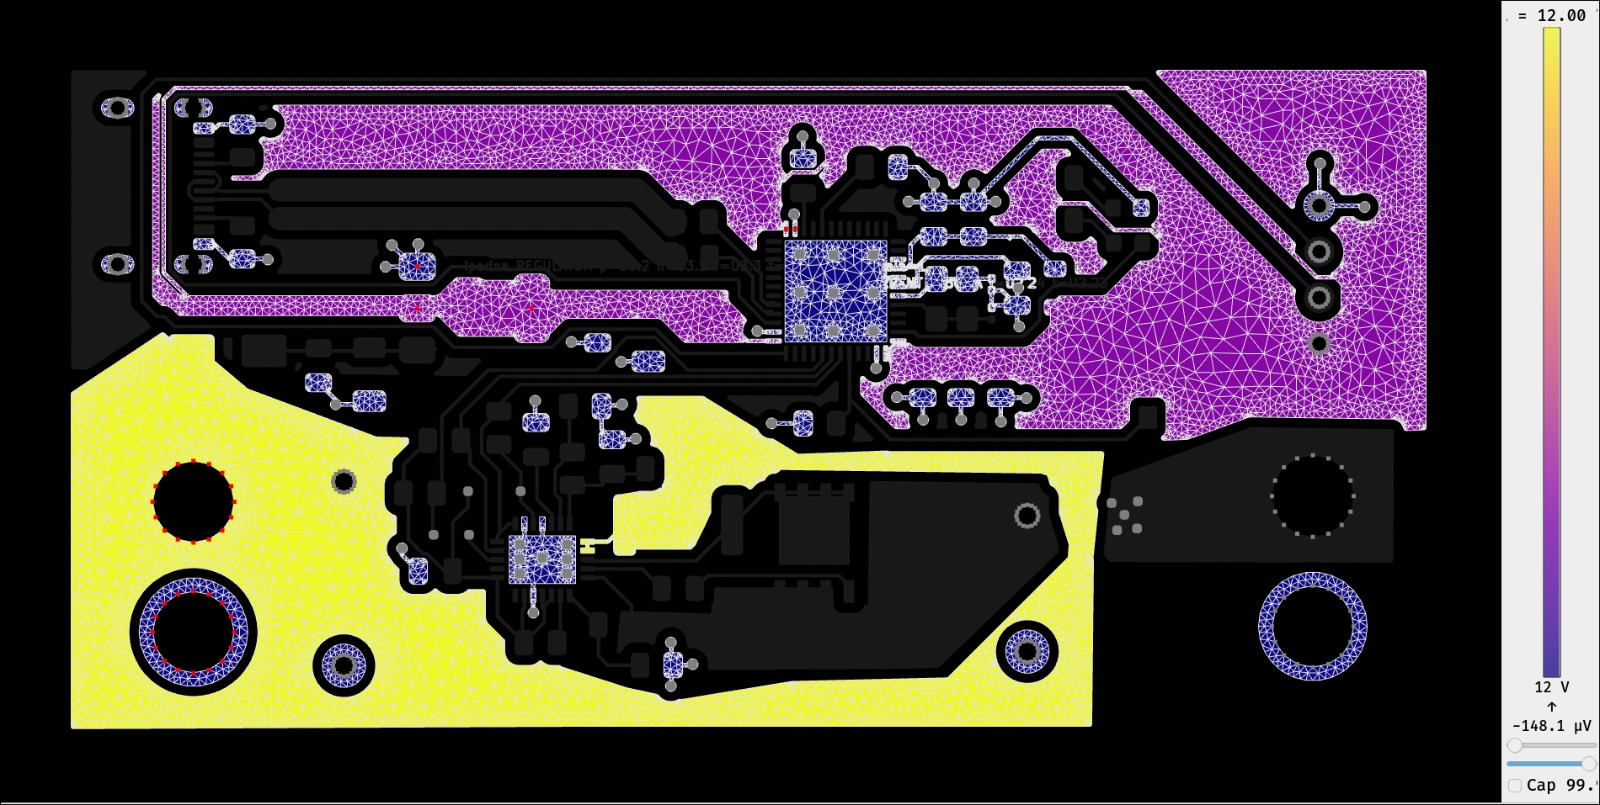
\includegraphics[width=0.85\textwidth]{figures/pdn_dc_voltage.png}
\caption{DC voltage distribution (\texttt{padne}): yellow/red = \SI{12}{\volt} eFuse input, purple =
3.3\,V/GND plane under the STM32's \SI{50}{\milli\ampere} load. The mesh triangulation is
\texttt{padne}'s FEM discretization of the copper pours.}
\label{fig:pdn-dc}
\end{figure}

\textbf{AC tooling note:} the AC sweep is planned with KiPI (github.com/drewsum/KiPI -- not the
similarly-named KiPIDA, which is DC-only). Getting it running exposed a real packaging gap: its
\texttt{requirements.txt} pins \texttt{triangle>=20230923}, a meshing dependency with no published
wheel past CPython 3.12 and no source distribution on PyPI, so the install silently stalled on newer
Python. Worked around by building \texttt{triangle} from its GitHub source directly into KiPI's
plugin-managed virtual environment.

% ======================================================================
\section{Known Limitations}

\begin{itemize}
\item \textbf{No firmware written or tested.} The I\textsuperscript{2}C telemetry path (SDA/SCL/ALERT)
  is wired and DRC-clean, but nothing has read a register from the LTC4215 yet, real or simulated.
\item \textbf{LTC4215 is not PMBus-compliant.} It has its own proprietary I\textsuperscript{2}C
  register map (datasheet Tables 2/3), not the standardized PMBus command set. This project is
  "digital power monitoring in the spirit of PMBus," not a PMBus device, and is described that way
  deliberately to avoid overstating the IC's actual capability.
\item \textbf{Simulation/layout only, not built} -- same as every project in this series; no bring-up
  measurements exist for any of the new circuitry (LDO, USB PHY, I\textsuperscript{2}C timing).
\end{itemize}
\label{sec:scope-thermal}
No new thermal analysis was performed for this revision. The LDO's estimated \SI{0.42}{\watt} at an
assumed \SI{50}{\milli\ampere} load is a hand estimate, not simulated; the eFuse power stage's
thermal behavior (R5/Q1 at \SI{12}{\volt}/\SI{15}{\ampere}) was already characterized in
\texttt{EFUSE\_LTC4215} and is unchanged by this addition.

% ======================================================================
\section{Pending}
\label{sec:pending}

\begin{pending}
\begin{itemize}
\item Firmware: an I\textsuperscript{2}C driver reading the LTC4215's ADIN/status/fault registers per
  the datasheet's command table, converting raw ADC counts to real current/voltage. To be verified by
  (a) compiling cleanly against the STM32F411 HAL, and (b) a host-side unit test feeding it synthetic
  register bytes constructed from the datasheet's own description, \emph{not} by claiming it was
  tested on real hardware -- this board was never built.
\item PDN AC impedance-vs-frequency sweep of the 3.3\,V rail and its decoupling bank (DC voltage-drop
  check already done, Section~\ref{sec:pdn}), to confirm the capacitor values chosen by convention
  actually cover the relevant frequency range rather than just assuming "\SI{100}{\nano\farad} near
  every pin is enough." Tooling (KiPI) is installed and loads the board; the probe/sweep setup was not
  finished this session.
\item A permanent fix for the crystal's pad 3/4 net assignment being wiped on every schematic re-sync
  (either edit the symbol's own pin-to-pad mapping in a local library copy, or simply stop re-running
  "Update PCB from Schematic" now that the schematic is stable).
\item If continuous \SI{15}{\ampere} operation is ever revisited: same open item as
  \texttt{EFUSE\_LTC4215} (heavier copper, metal-strip sense resistor, or airflow) -- unaffected by
  this addition.
\end{itemize}
\end{pending}

% ======================================================================
\section{Conclusions}

A minimal STM32F411CEU6 system was added to the LTC4215 eFuse board specifically to exercise the
I\textsuperscript{2}C monitoring interface that the original design had left wired open -- SDAI/SDAO
tied per the datasheet, the device address reproduced from the datasheet's own worked example rather
than invented, and pull-ups referenced to INTVCC after confirming its regulated voltage is close
enough to 3.3\,V logic levels to skip a level shifter. The MCU side follows the real WeAct Blackpill
reference schematic where it was correct and departs from it where it was not: no RTC battery/crystal
(not needed here), a single-stage 12\,V-direct LDO instead of the Blackpill's two-stage USB-fed supply
(this board is never USB-powered), and an independently re-derived, datasheet-confirmed need for the
BOOT1 pull-down that was initially (incorrectly) dismissed as an F1-series leftover.

The schematic and PCB are ERC/DRC-clean; the remaining DRC entries are inherent to the USB-C
connector footprint itself (NPTH hole clearance to its own mounting holes, and the four
intentionally-No-Connect VBUS pads touching each other) rather than unresolved design issues. Several
non-obvious layout pitfalls specific to this part -- the hidden/stacked VSS pins, the 4-pad crystal
footprint's two-terminal reality, same-net labels silently merging across unrelated blocks, and a
confirmed (not assumed) BOOT1 requirement on the F411 -- are documented in
Section~\ref{sec:pitfalls} for the next project that touches this MCU family.

Firmware and a PDN impedance check remain open, both scoped honestly in Section~\ref{sec:pending}
rather than claimed as done.

\end{document}
